\section{Question 1}
\subsection{Équations du mouvement}
Soit le système hamiltonien à deux corps, d'invariant $\Ha (p,q)$ où $p$ est la vitesse de chaque corps et $q$ leur position
\footnote{On a évidemment $p(t)$ et $q(t)$. Pour une planète, la composante $p_1$ représente sa vitesse dans la direction ``$x$'' du plan et la composante $p_2$, sa vitesse dans la direction ``$y$'' du plan.}.
Considérons tout d'abord un système où un des deux corps a une masse considérablement plus élevée que l'autre, ce qui nous permet de le considérer comme statique. On a alors
$$\Ha (p,q) = \frac{1}{2} p^T p - \frac{1}{||q||_2} . $$
On sait que $\dot{\Ha}(p,q) = 0$ car $\Ha$ est invariant dans le temps.
De plus, comme (par la règle de dérivée en chaîne)
\[
  \dot{\Ha}(p,q) = \fpart{\Ha(p,q)}{p}^T\dot{p} + \fpart{\Ha(p,q)}{q}^T\dot{q},
\]
on doit avoir
\[
  \fpart{\Ha(p,q)}{q}^T\dot{q} + \fpart{\Ha(p,q)}{p}^T\dot{p} = 0.
\]

Les équations
\begin{align*}
  \dot{q} & = \fpart{\Ha(p,q)}{p} & \dot{p} & = -\fpart{\Ha(p,q)}{q}
\end{align*}
donnent
\begin{align*}
  \fpart{\Ha(p,q)}{q}^T\dot{q} + \fpart{\Ha(p,q)}{p}^T\dot{p} & =
  \fpart{\Ha(p,q)}{q}^T\fpart{\Ha(p,q)}{p} - \fpart{\Ha(p,q)}{p}^T\fpart{\Ha(p,q)}{q}\\
  & = 0
\end{align*}
ce qui respecte bien l'invariance temporelle de $\Ha$.

Soient $f_1(q,p)$ et $f_2(q,p)$ tels que
\begin{align*}
  \dot{q} & = f_1(q,p)\\
  \dot{p} & = f_2(q,p),
\end{align*}
on calcule
\begin{align*}
  f_1(q,p) & =  \fpart{\Ha (p,q)}{p}\\
  & =
  \begin{pmatrix}
    \fpart{}{p_1} \left(\frac{1}{2}(p_1^2 + p_2^2) - \frac{1}{\sqrt{q_1^2 + q_2^2}}\right)\\
    \fpart{}{p_2} \left(\frac{1}{2}(p_1^2 + p_2^2) - \frac{1}{\sqrt{q_1^2 + q_2^2}}\right)
  \end{pmatrix}\\
  & =
  \begin{pmatrix}
    p_1\\
    p_2
  \end{pmatrix}\\
  & = p\\
%
  f_2(q,p) & =  -\fpart{\Ha (p,q)}{q}\\
  & =
  -\begin{pmatrix}
    \fpart{}{q_1} \left(\frac{1}{2}(p_1^2 + p_2^2) - \frac{1}{\sqrt{q_1^2 + q_2^2}}\right)\\
    \fpart{}{q_2} \left(\frac{1}{2}(p_1^2 + p_2^2) - \frac{1}{\sqrt{q_1^2 + q_2^2}}\right)
  \end{pmatrix}\\
  & =
  \frac{-1}{2(q_1^2 + q_2^2)^{3/2}}
  \begin{pmatrix}
    2q_1\\
    2q_2
  \end{pmatrix}\\
  & = \frac{-q}{\|q\|_2^3}
\end{align*}
ce qui n'est guère étonnant pour $\dot{q} = p$ car comme $q$ est la position,
$\dot{q}$ est la vitesse, c'est à dire $p$.

Les équations du mouvement sont donc données par :
\begin{equation} \label{equation_mvt}
\left\lbrace
\begin{array}{ccc}
\dot{q} &=& p\\
\dot{p} &=&  \frac{-q}{\|q\|_2^3}
\end{array}
\right.
\end{equation}

Ce système d'équations différentielles admet une unique solution dans $\mathbb{R}_0^4$. En effet :
\begin{eqnarray}
||f_1(x)-f_1(y)|| &\leq & ||x-y|| \\
||f_2(x) - f_2(y)|| &\leq & \left\|\frac{x}{\|x\|_2^3} - \frac{y}{\|y\|_2^3}\right\| \leq \max(\frac{1}{\|x\|_2^3}, \frac{1}{\|y\|_2^3}) ||x-y||.
\end{eqnarray}
Ce qui implique que le système est Lipschitzien et, par le théorème 5.1 du cours, le système \ref{equation_mvt} admet une unique solution.

\subsection{Description des méthodes numériques}
Nous souhaitons intégrer ce système d'équations différentielles non-linéaires (de forme générale $y'(t) = f(t,y)$, où $y$ désigne aussi bien un scalaire qu'un vecteur) par les méthodes numériques suivantes :
\begin{itemize}
\item la méthode d'Euler explicite, $y_{n+1} = y_n + h f(t,y_n)$
\item la méthode d'Euler implicite, $y_{n+1} = y_n + h f(t,y_{n+1})$ qui demande de résoudre une équation non-linéaire de type $g(y_{n+1})=0$ à chaque itération, qu'on résoudra en utilisant la méthode itérative de Newton-Raphson
\item la méthode d'Euler symplectique qui est une combinaison des méthodes d'Euler implicite et explicite (on applique le schéma implicite à une composante de $y$ et un schéma explicite à l'autre).
\end{itemize}

On remarque que $f_1(q,p) = f_1(p)$ et $f_2(q,p) = f_2(q)$.
On va utiliser cette propriété qui va nous être particulièrement utile pour Euler symplectique.
Pour Euler implicite, on aura besoin de
\begin{align*}
  \fpart{f_1(p)}{p} & = I\\
  \fpart{f_2(q)}{q} & =
  \begin{pmatrix}
    \fpart{}{q_1}\frac{-q_1}{(q_1^2 + q_2^2)^{3/2}} &
    \fpart{}{q_2}\frac{-q_1}{(q_1^2 + q_2^2)^{3/2}}\\
    \fpart{}{q_1}\frac{-q_2}{(q_1^2 + q_2^2)^{3/2}} &
    \fpart{}{q_2}\frac{-q_2}{(q_1^2 + q_2^2)^{3/2}}
  \end{pmatrix}\\
  & =
  \begin{pmatrix}
    \frac{-(q_1^2 + q_2^2)^{3/2} + 3q_1^2(q_1^2 + q_2^2)^{1/2}}{(q_1^2 + q_2^2)^3} &
    \frac{3q_1q_2}{(q_1^2 + q_2^2)^{5/2}}\\
    \frac{3q_1q_2}{(q_1^2 + q_2^2)^{5/2}} &
    \frac{-(q_1^2 + q_2^2)^{3/2} + 3q_2^2(q_1^2 + q_2^2)^{1/2}}{(q_1^2 + q_2^2)^3}
  \end{pmatrix}\\
  & =
  \begin{pmatrix}
    \frac{2q_1^2 - q_2^2}{(q_1^2 + q_2^2)^{5/2}} &
    \frac{3q_1q_2}{(q_1^2 + q_2^2)^{5/2}}\\
    \frac{3q_1q_2}{(q_1^2 + q_2^2)^{5/2}} &
    \frac{-q_1^2 + 2q_2^2}{(q_1^2 + q_2^2)^{5/2}}
  \end{pmatrix}\\
  & =
  \frac{1}{\|q\|_2^{5}}
  \begin{pmatrix}
    2q_1^2 - q_2^2 &
    3q_1q_2\\
    3q_1q_2 &
    -q_1^2 + 2q_2^2
  \end{pmatrix}
\end{align*}

L'équation que Newton-Raphson devra résoudre à chaque pas est la suivante
\begin{align*}
  q_{k+1} & = q_k + hf_1(p_{k+1})\\
  p_{k+1} & = p_k + hf_2(q_{k+1})
\end{align*}
ou encore
\begin{align*}
  q_k - q_{k+1} + hf_1(p_{k+1}) & = 0\\
  p_k + hf_2(q_{k+1}) - p_{k+1} & = 0
\end{align*}
On doit donc résoudre $g(u) = 0$ où
$u =
\begin{pmatrix}
  q_{k+1}\\
  p_{k+1}
\end{pmatrix}$
et
\[
  g
  \left(
    \begin{pmatrix}
      q_{k+1}\\
      p_{k+1}
    \end{pmatrix}
  \right) =
  \begin{pmatrix}
    q_k - q_{k+1} + hf_1(p_{k+1})\\
    p_k + hf_2(q_{k+1}) - p_{k+1}
  \end{pmatrix}
\]
d'où
\[
  \fpart{g}{u}
  \left(
    \begin{pmatrix}
      q_{k+1}\\
      p_{k+1}
    \end{pmatrix}
  \right) =
  \begin{pmatrix}
    -I & h\fpart{f_1}{p}(p_{k+1})\\
    h\fpart{f_2}{q}(q_{k+1}) & -I
  \end{pmatrix}.
\]


\subsection{Comparaison des méthodes numériques}

Appliquons a présent ces méthodes sur un cas concret où la planète mobile a comme caractéristiques initiales : $p_0 = \begin{pmatrix}
0\\
2
\end{pmatrix}
$ et $q_0 = \begin{pmatrix}
0.4\\
0
\end{pmatrix}
$.\\

Nous allons appliquer à ce cas les différentes méthodes d'intégration numérique pour 100 000 pas de temps dont la valeur est $h=5e-4$ (Euler implicite et explicite) ou $h=5e-2$ (Euler symplectique). Les résultats sont donnés aux figures \ref{fig:q1_exp}, \ref{fig:q1_imp} et \ref{fig:q1_sym}.

\begin{figure}[!ht]
  \centering
  \begin{subfigure}[b]{0.45\textwidth}
    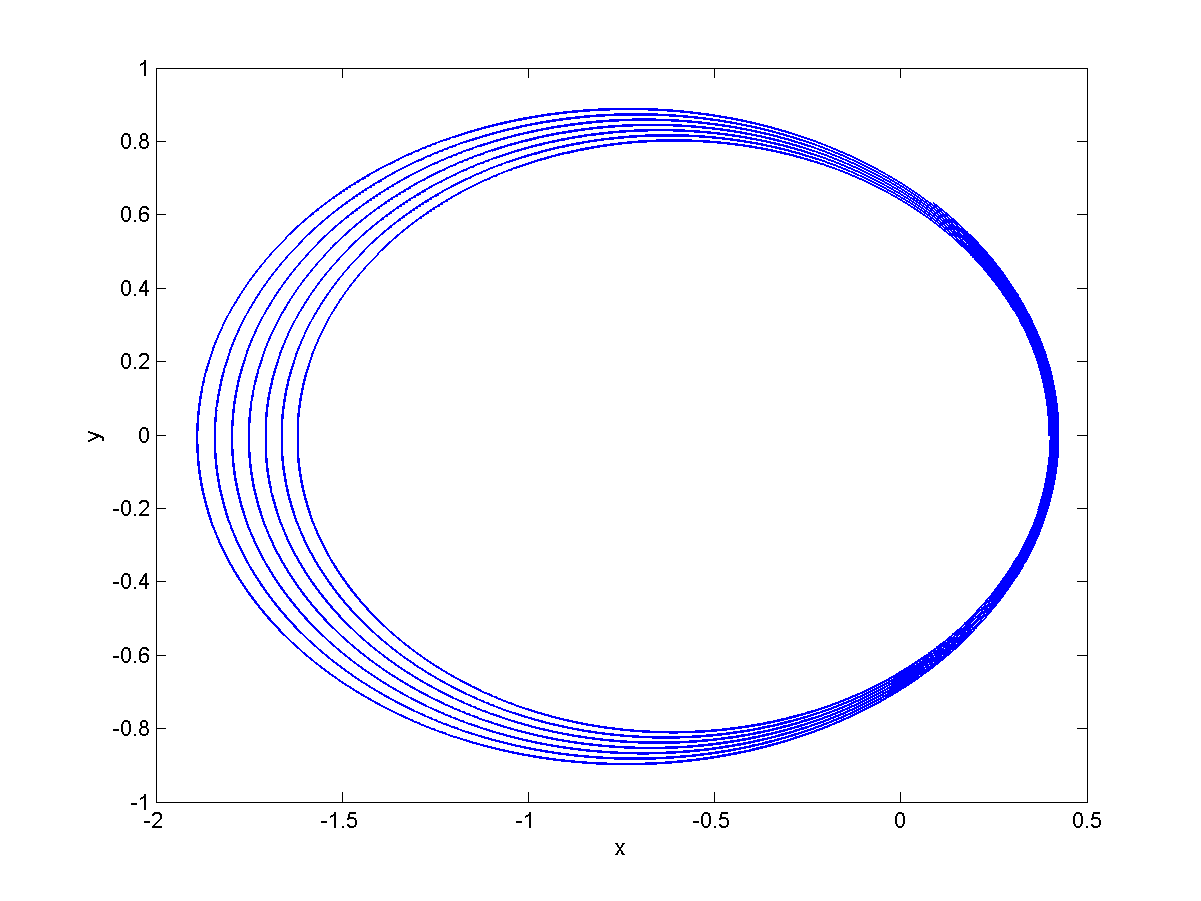
\includegraphics[width=\textwidth]{images/Q1_explicite_q.png}
    \caption{$q$ pour explicite}
    \label{fig:q1_explicite_q}
  \end{subfigure}%
  \begin{subfigure}[b]{0.45\textwidth}
    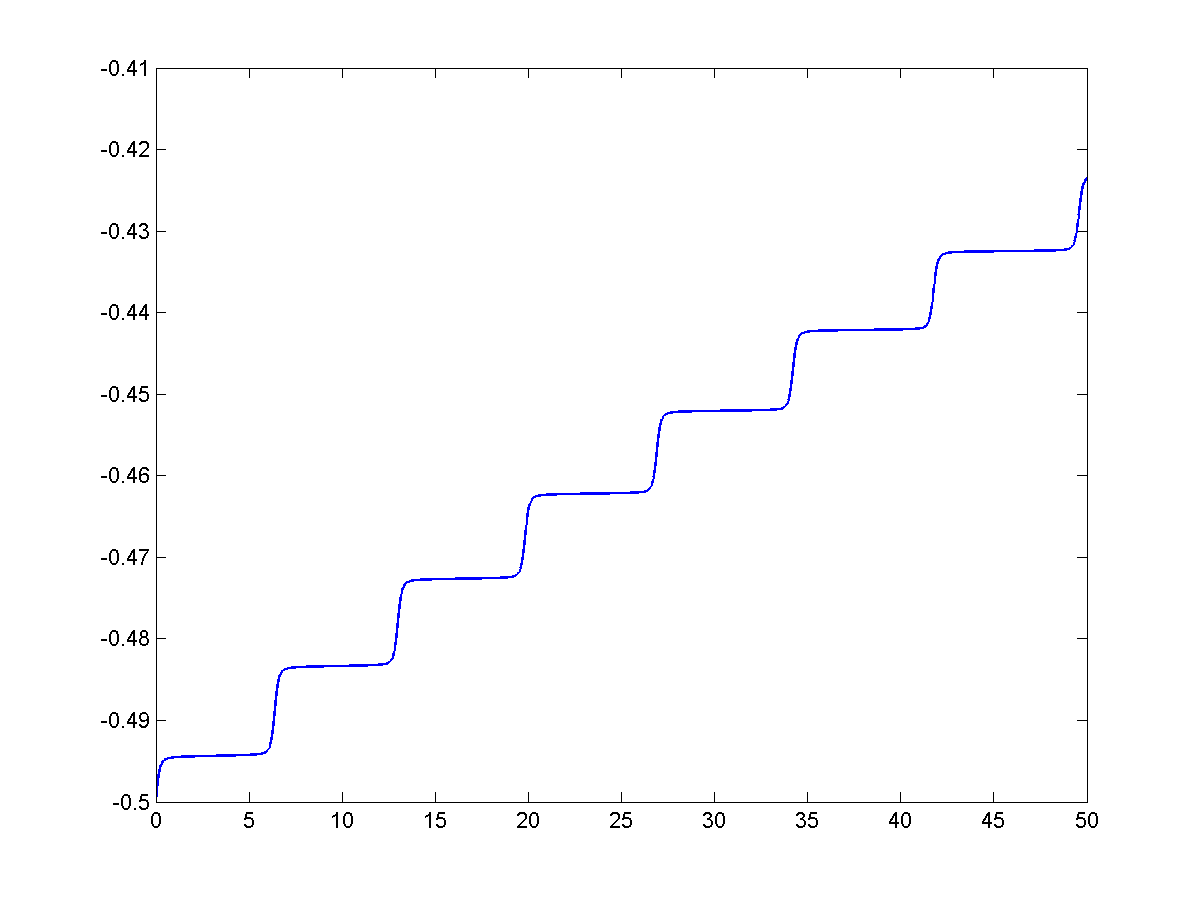
\includegraphics[width=\textwidth]{images/Q1_explicite_H.png}
    \caption{$\Ha$ pour explicite}
    \label{fig:q1_explicite_H}
  \end{subfigure}
  \begin{subfigure}[b]{0.45\textwidth}
    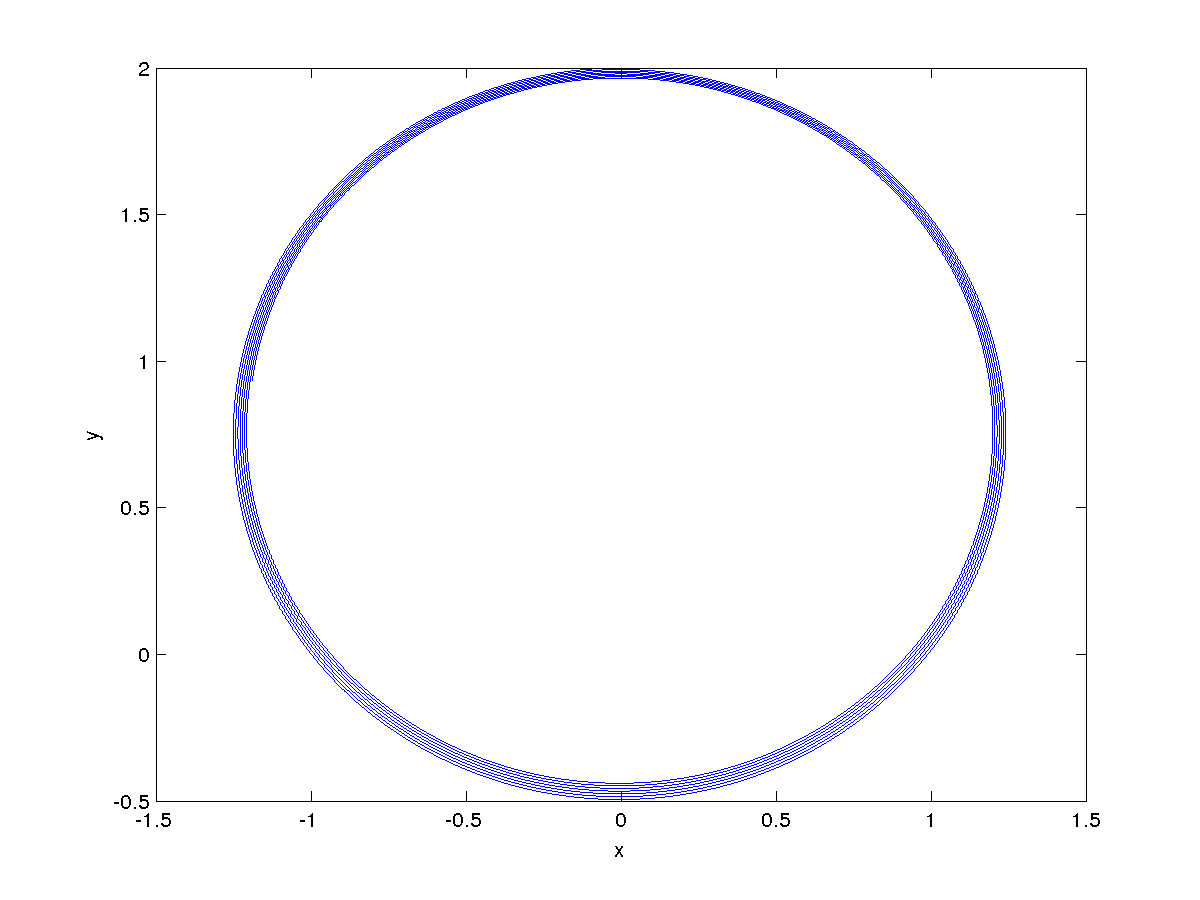
\includegraphics[width=\textwidth]{images/Q1_explicite_p.png}
    \caption{$p$ pour explicite}
    \label{fig:q1_explicite_p}
  \end{subfigure}
  \begin{subfigure}[b]{0.45\textwidth}
    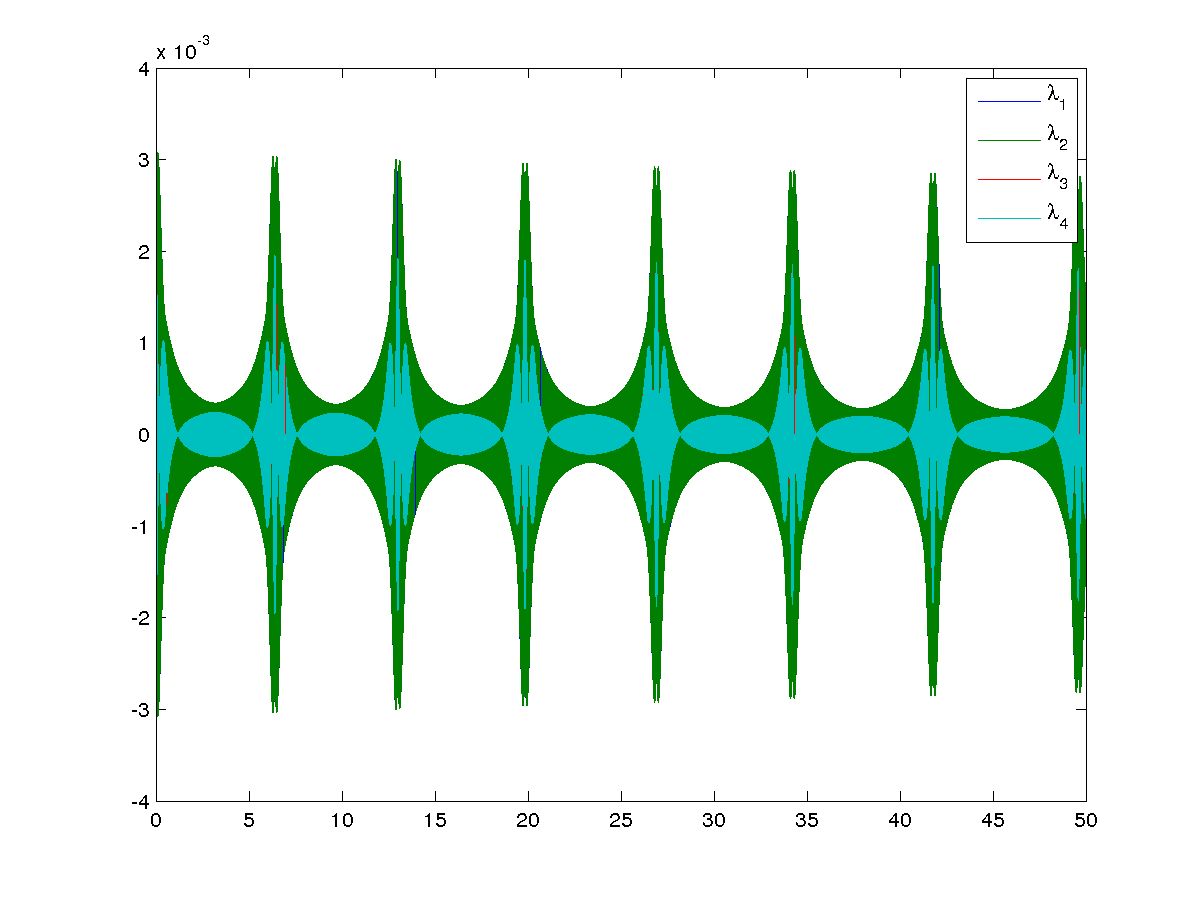
\includegraphics[width=\textwidth]{images/Q1_explicite_lambda.png}
    \caption{$h\lambda$ en fonction du temps pour explicite}
    \label{fig:q1_explicite_lambda}
  \end{subfigure}
  \caption{Résultats pour la question 1 pour Euler explicite}
  \label{fig:q1_exp}
\end{figure}

\begin{figure}[!ht]
  \begin{subfigure}[b]{0.45\textwidth}
    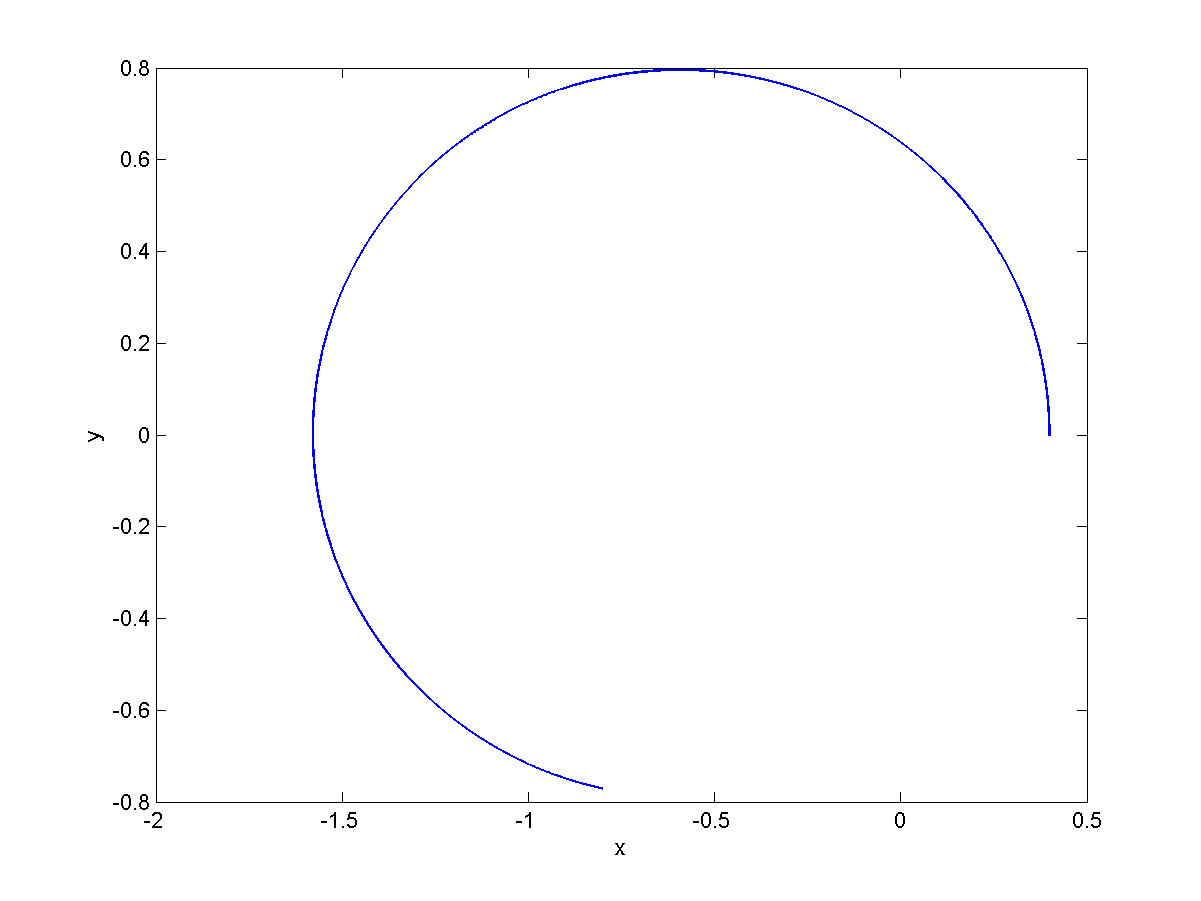
\includegraphics[width=\textwidth]{images/Q1_implicite_q.png}
    \caption{$q$ pour implicite}
    \label{fig:q1_implicite_q}
  \end{subfigure}%
  \begin{subfigure}[b]{0.45\textwidth}
    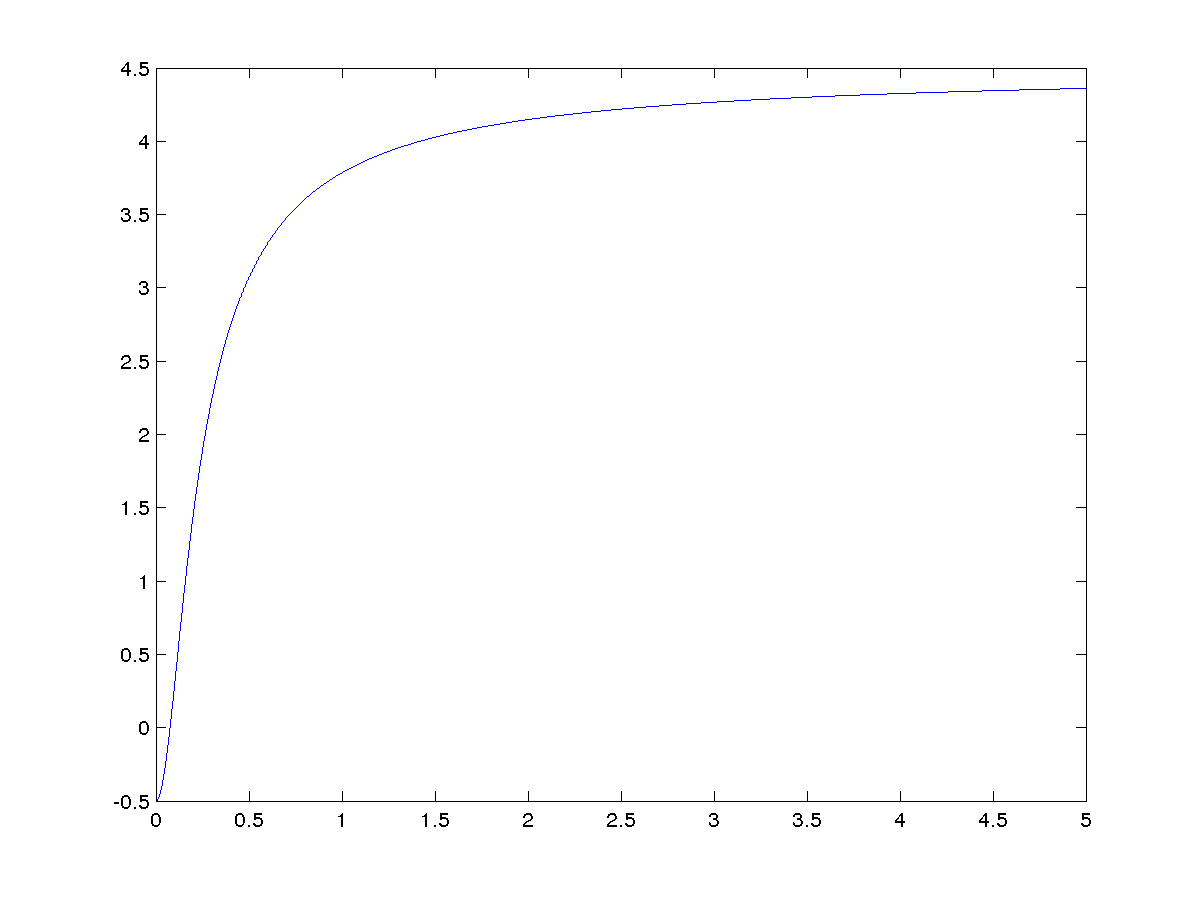
\includegraphics[width=\textwidth]{images/Q1_implicite_H.png}
    \caption{$\Ha$ pour implicite}
    \label{fig:q1_implicite_H}
  \end{subfigure}
  \begin{subfigure}[b]{0.45\textwidth}
    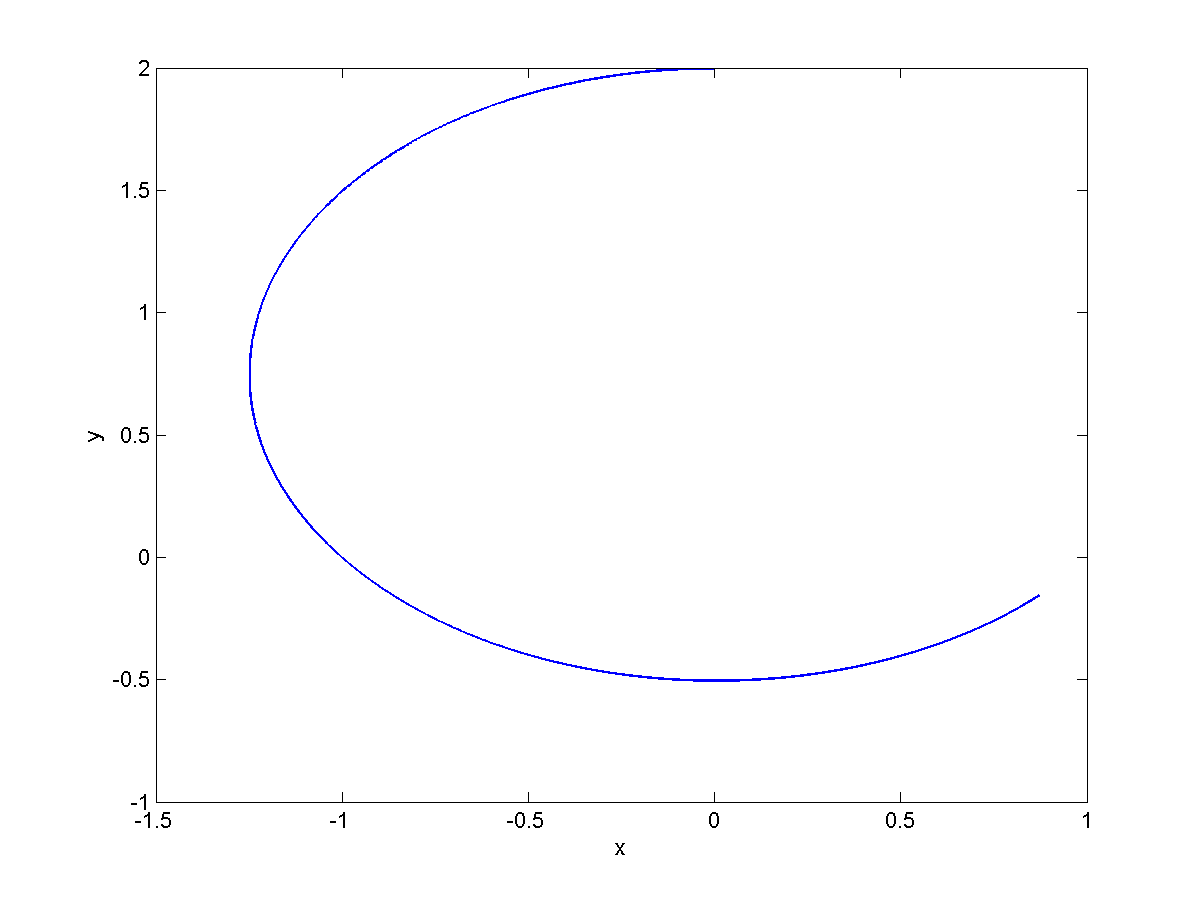
\includegraphics[width=\textwidth]{images/Q1_implicite_p.png}
    \caption{$p$ pour implicite}
    \label{fig:q1_implicite_p}
  \end{subfigure}
  \begin{subfigure}[b]{0.45\textwidth}
    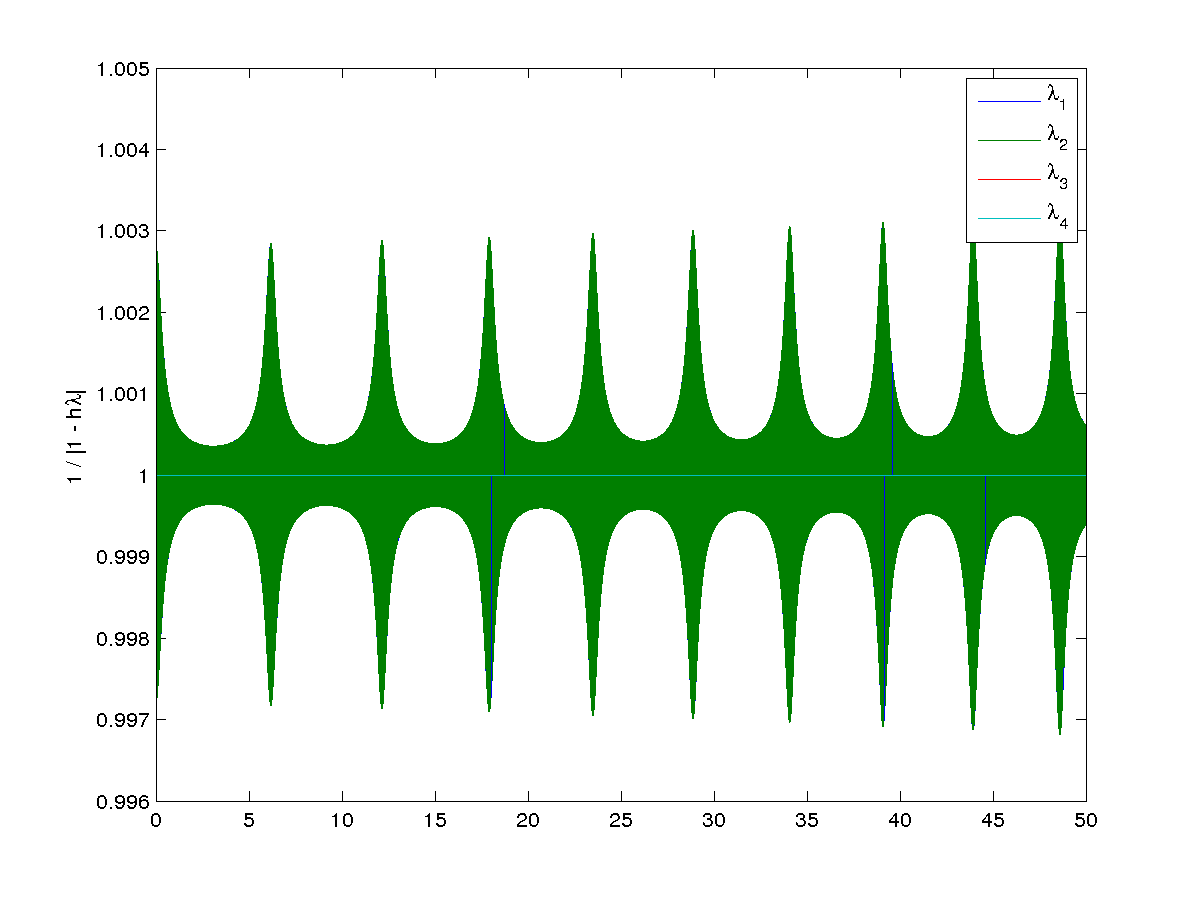
\includegraphics[width=\textwidth]{images/Q1_implicite_lambda.png}
    \caption{$h\lambda$ en fonction du temps pour implicite}
    \label{fig:q1_implicite_lambda}
  \end{subfigure}
  \caption{Résultats pour la question 1 pour Euler implicite}
  \label{fig:q1_imp}
\end{figure}

\begin{figure}[!ht]
  \centering
  \begin{subfigure}[b]{0.3\textwidth}
    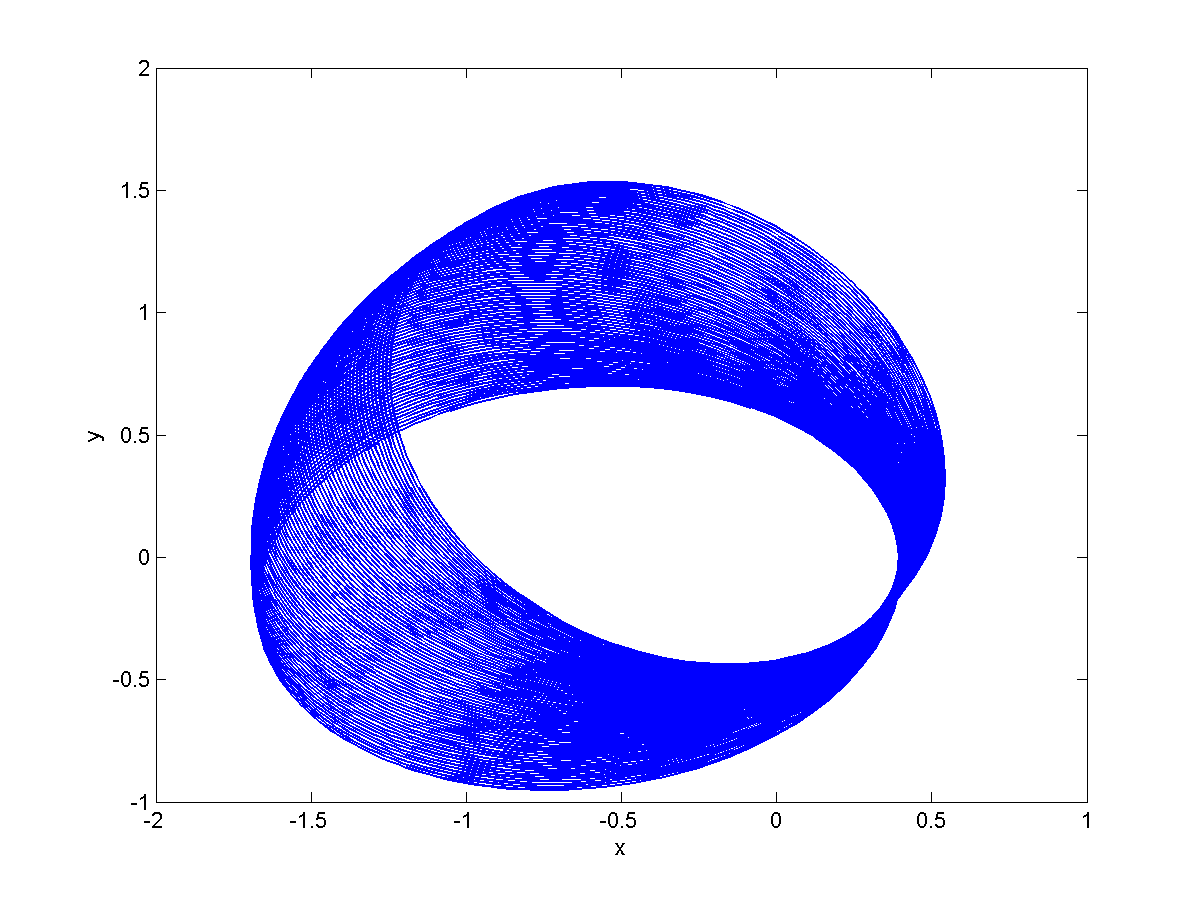
\includegraphics[width=\textwidth]{images/Q1_symplectique1_q.png}
    \caption{$q$ pour symplectique1}
    \label{fig:q1_symplectique1_q}
  \end{subfigure}%
  ~
  %(or a blank line to force the subfigure onto a new line)
  \begin{subfigure}[b]{0.3\textwidth}
    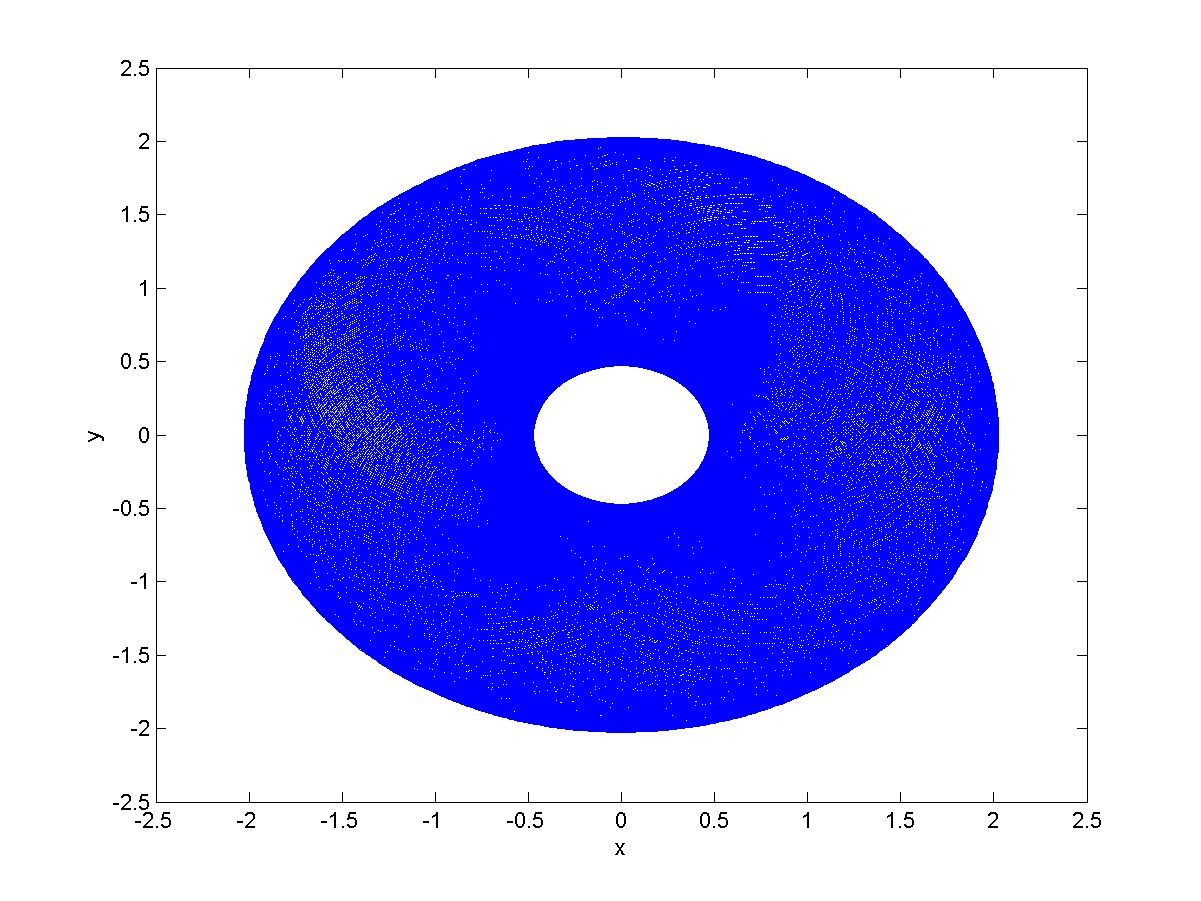
\includegraphics[width=\textwidth]{images/Q1_symplectique1_p.png}
    \caption{$p$ pour symplectique1}
    \label{fig:q1_symplectique1_p}
  \end{subfigure}
  ~
  \begin{subfigure}[b]{0.3\textwidth}
    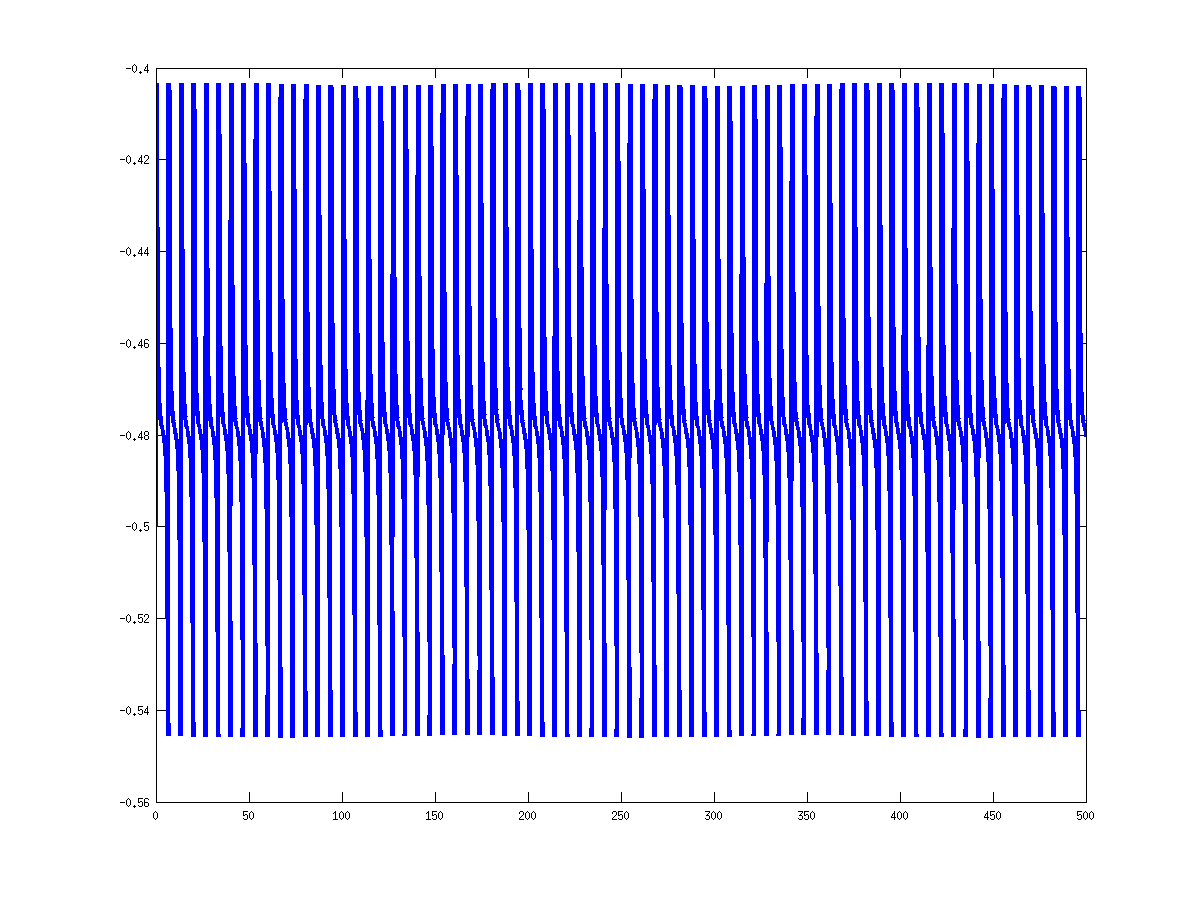
\includegraphics[width=\textwidth]{images/Q1_symplectique1_H.png}
    \caption{$\Ha$ pour symplectique1}
    \label{fig:q1_symplectique1_H}
  \end{subfigure}

  \begin{subfigure}[b]{0.3\textwidth}
    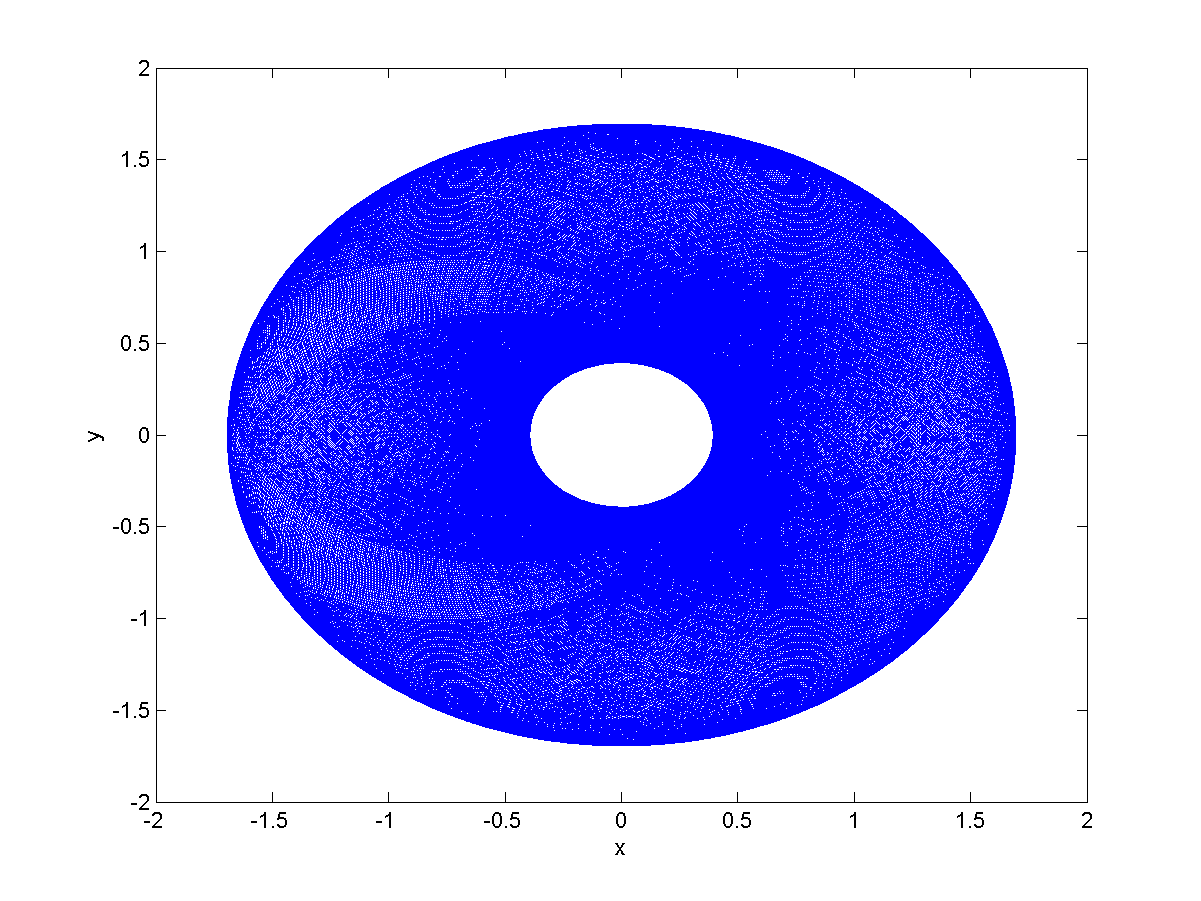
\includegraphics[width=\textwidth]{images/Q1_symplectique2_q.png}
    \caption{$q$ pour symplectique2}
    \label{fig:q1_symplectique2_q}
  \end{subfigure}%
  ~
  %(or a blank line to force the subfigure onto a new line)
  \begin{subfigure}[b]{0.3\textwidth}
    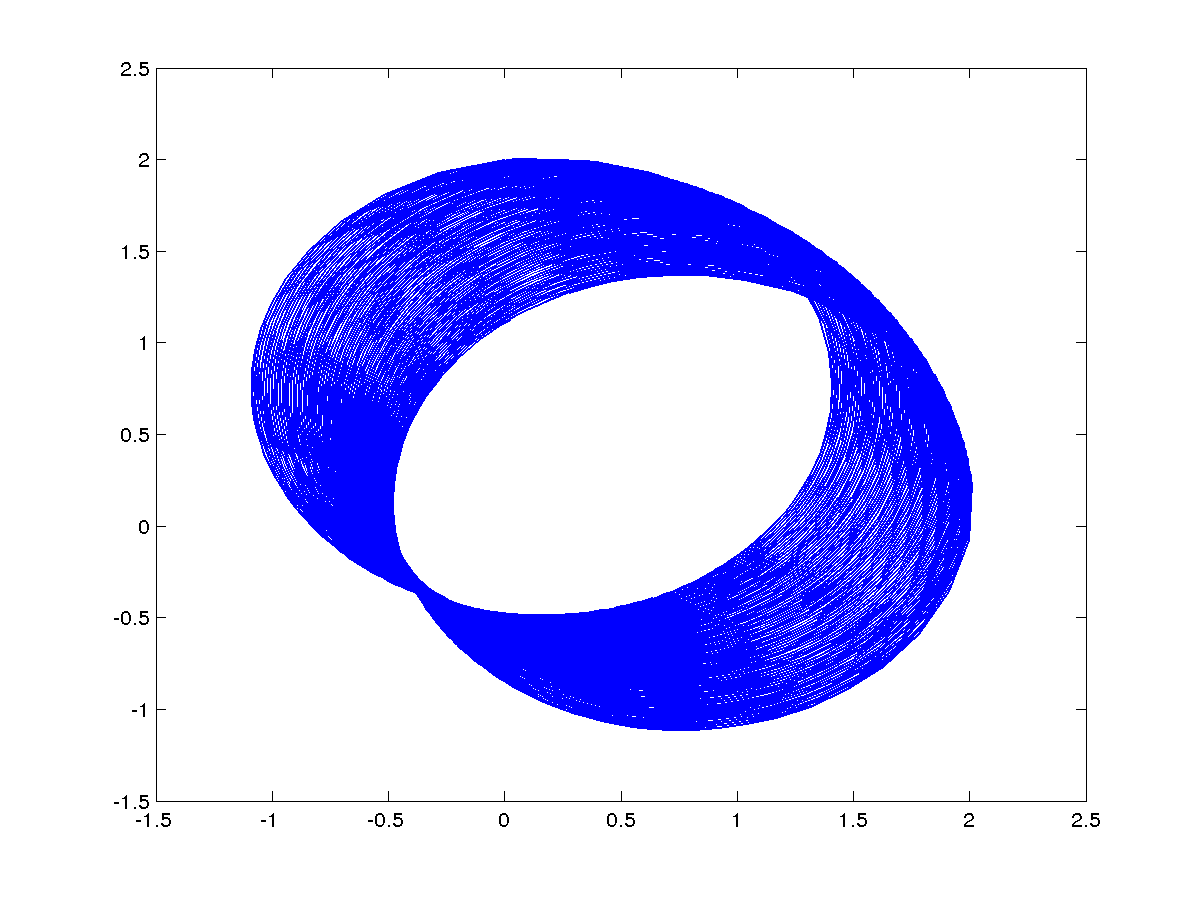
\includegraphics[width=\textwidth]{images/Q1_symplectique2_p.png}
    \caption{$p$ pour symplectique2}
    \label{fig:q1_symplectique2_p}
  \end{subfigure}
  ~
  \begin{subfigure}[b]{0.3\textwidth}
    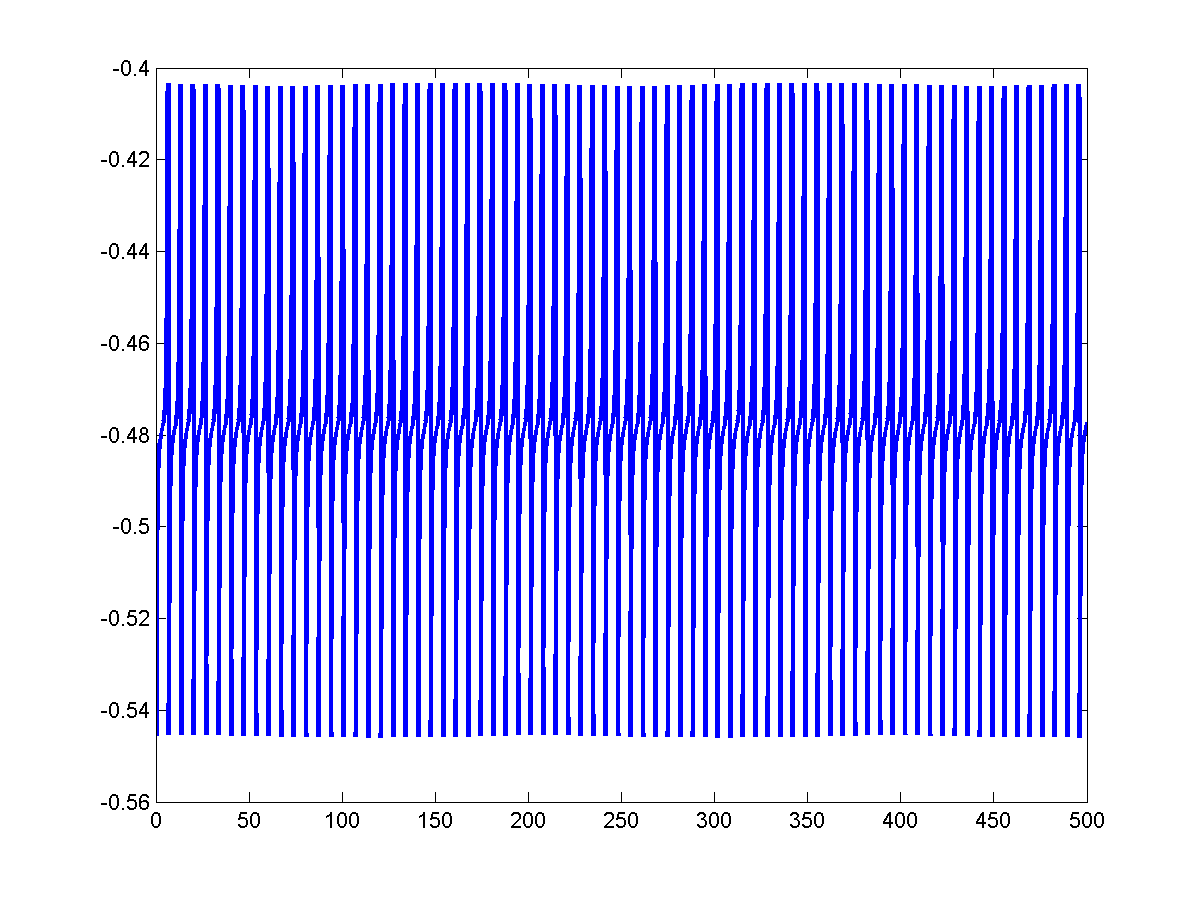
\includegraphics[width=\textwidth]{images/Q1_symplectique2_H.png}
    \caption{$\Ha$ pour symplectique2}
    \label{fig:q1_symplectique2_H}
  \end{subfigure}
  \caption{Résultats pour la question 1 pour Euler symplectique}
  \label{fig:q1_sym}
\end{figure}


Les principaux points de comparaison des méthodes sont la convergence, l'erreur et le temps de calcul de la méthode.

\subsubsection{Convergence}
Pour étudier la convergence, nous aurons besoin de la Jacobienne :
$$J(q,p) =
\begin{pmatrix}
  0 & 0 & 1 & 0\\
  0 & 0 & 0 & 1\\\\
  \frac{2q_1^2 - q_2^2}{(q_1^2+q_2^2)^{5/2}} & \frac{3q_1q_2}{(q_1^2+q_2^2)^{5/2}} & 0 & 0 \\
  \frac{3q_1q_2}{(q_1^2+q_2^2)^{5/2}} & \frac{2q_2^2 - q_1^2}{(q_1^2+q_2^2)^{5/2}} & 0 & 0
\end{pmatrix}.
$$
Pour rappel, l'erreur entre la ``vraie'' solution d'une équation différentielle ordinaire et celle obtenue pour des conditions initiales perturbée est définie comme :
$$\left\lbrace
\begin{array}{ccc}
e' &=& \lambda e\\
e(a) &=& \epsilon
\end{array}
\right.
$$
Où $\lambda$ est la jacobienne du système évaluée en un certain point. Le système sera donc stable si $\mathcal{R} (J) <0$. Pour un système d'équations différentielles, on a donc :
$$\left\lbrace
\begin{array}{ccc}
e' &=& A e\\
e(a) &=& \epsilon
\end{array}
\right.
$$
Si $A$ est diagonalisable, on peut effectuer un changement de variable tel que
$$\left\lbrace
\begin{array}{ccc}
\tilde{e} ' &=& D \tilde{e}\\
\tilde{e} (a) &=& \epsilon
\end{array}
\right.
$$
Où $D$ est la matrice diagonale des valeurs propres. On se retrouve alors avec $n$ équations différentielles découplées dont la condition de stabilité est $\mathcal{R} (\lambda_i) <0$; c'est-à-dire tel que toutes les valeurs propres de la jacobienne soient à gauche de l'axe imaginaire.\\
On voit directement que notre système n'est pas stable. En effet, calculons par exemple les valeurs propres au point de départ :
$$J(q,p) =
\begin{pmatrix}
0 & 0 & 1 & 0\\
0 & 0 & 0 & 1\\\\
 31.2500 & 0  & 0 & 0 \\
0 & 15.6250 & 0 & 0
\end{pmatrix}
\Longrightarrow \mathrm{eig}(J(p,q))=
\begin{pmatrix}
5.5902\\
-5.5902\\
3.9528\\
-3.9528
\end{pmatrix}
$$

Les résultats numériques des valeurs de $h \lambda$ à chaque itération (la jacobienne variant à chaque itération)
sont donnés à la figure~\ref{fig:hlambda}.
On voit clairement que ces valeurs sont en dehors des zones de convergence d'Euler explicite
(cercle de centre $(-1,0)$ et de rayon 1) ainsi que d'Euler implicite
(tout le plan excepté le cercle de centre $(1,0)$ et de rayon 1),
ce qui est bien naturel étant donné que l'équation analytique est elle-même instable.
Notons bien sûre que le modèle n'est pas purement et simplement instable.
En effet, comme la jacobienne dépend de $q$, il existe des zones de stabilité et des zones d'instabilité.
Ce qui explique pourquoi le modèle n'explose pas après quelques itérations.

\begin{figure}
  \centering
  \begin{subfigure}[b]{0.5\textwidth}
    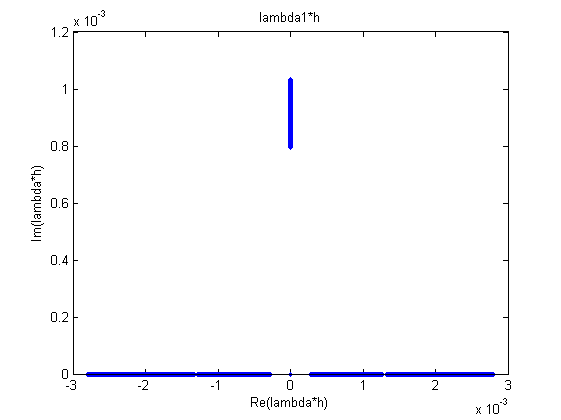
\includegraphics[width=\textwidth]{images/Q1_hlambda1.png}
    \caption{$h \lambda_1$}
  \end{subfigure}%
  ~ %add desired spacing between images, e. g. ~, \quad, \qquad etc.
  %(or a blank line to force the subfigure onto a new line)
  \begin{subfigure}[b]{0.5\textwidth}
    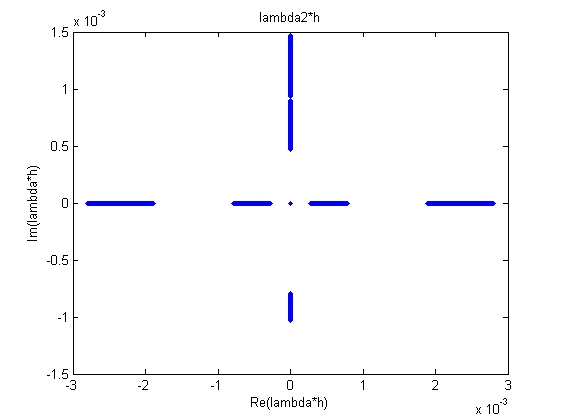
\includegraphics[width=\textwidth]{images/Q1_hlambda2.png}
    \caption{$h \lambda_2$}
  \end{subfigure}
  \begin{subfigure}[b]{0.5\textwidth}
    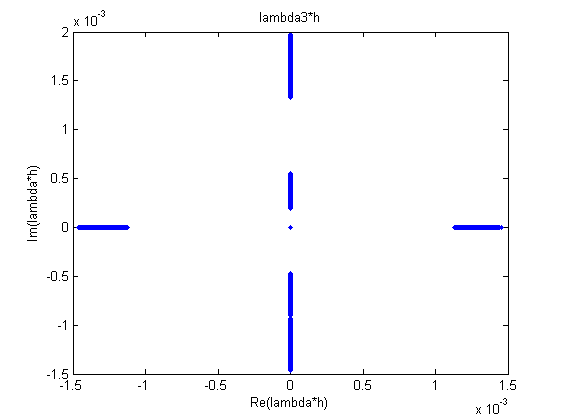
\includegraphics[width=\textwidth]{images/Q1_hlambda3.png}
    \caption{$h \lambda_3$}
  \end{subfigure}%
  ~
  %(or a blank line to force the subfigure onto a new line)
  \begin{subfigure}[b]{0.5\textwidth}
    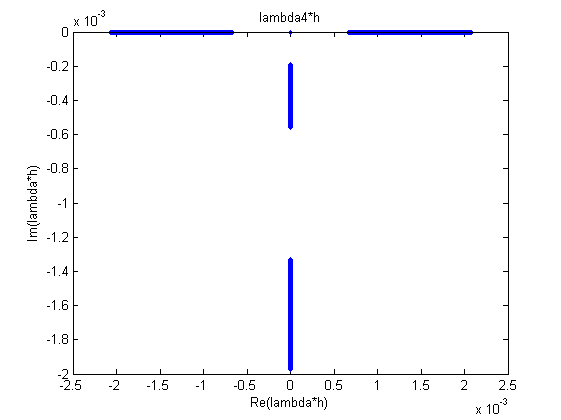
\includegraphics[width=\textwidth]{images/Q1_hlambda4.png}
    \caption{$h \lambda_4$}
  \end{subfigure}
  \caption{Valeurs de $h \lambda_i$ dans le plan complexe ($h=5e-4$).}
  \label{fig:hlambda}
\end{figure}

Que se passe-t-il si on prend un pas $h$ trop grand?
Les valeurs propres tendent toutes vers 0 et on obtient les résultats de la figure~\ref{fig_rater}.

\begin{figure}
  \centering
  \begin{subfigure}[b]{0.3\textwidth}
    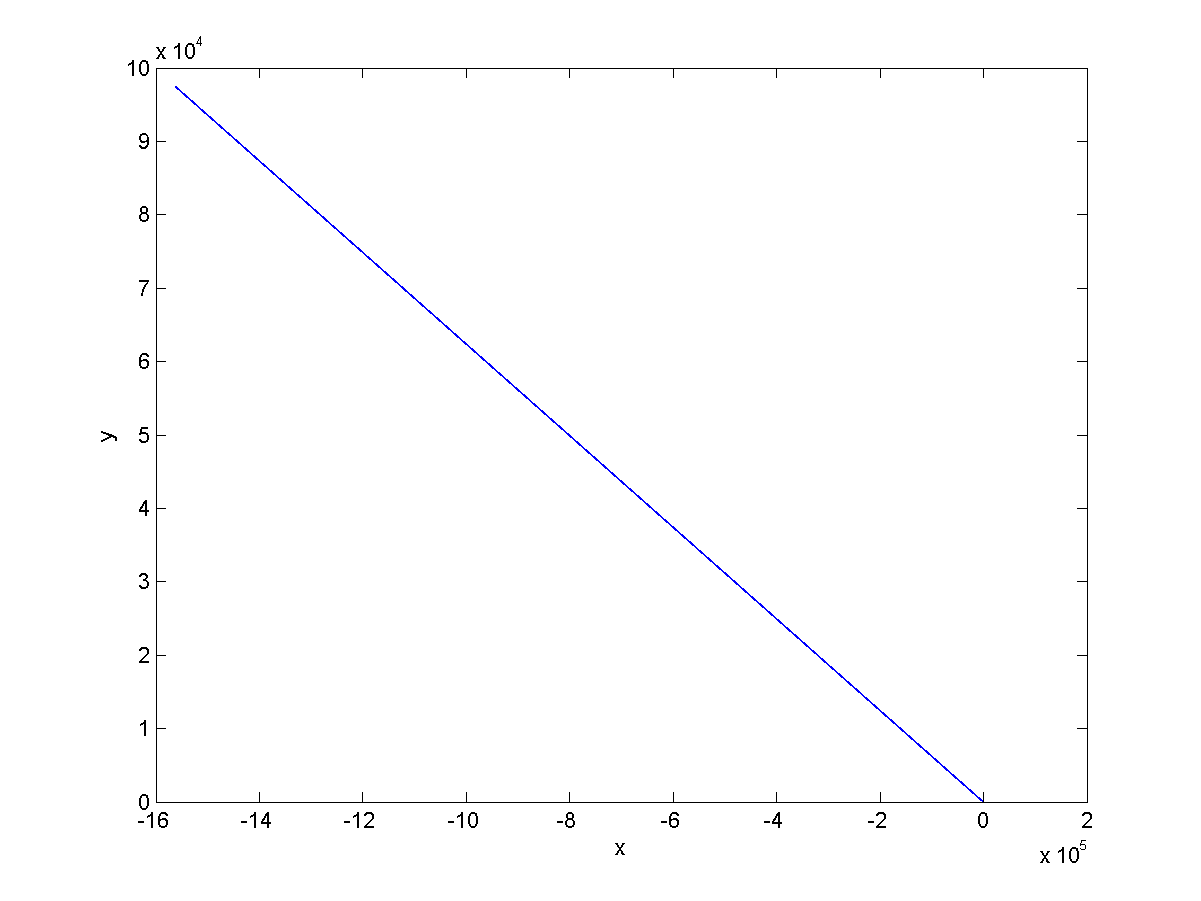
\includegraphics[width=\textwidth]{images/Q1_explicite_rate_q.png}
    \caption{$q$ pour explicite}
    \label{fig:q1_explicite_rate_q}
  \end{subfigure}%
  ~ %add desired spacing between images, e. g. ~, \quad, \qquad etc.
  %(or a blank line to force the subfigure onto a new line)
  \begin{subfigure}[b]{0.3\textwidth}
    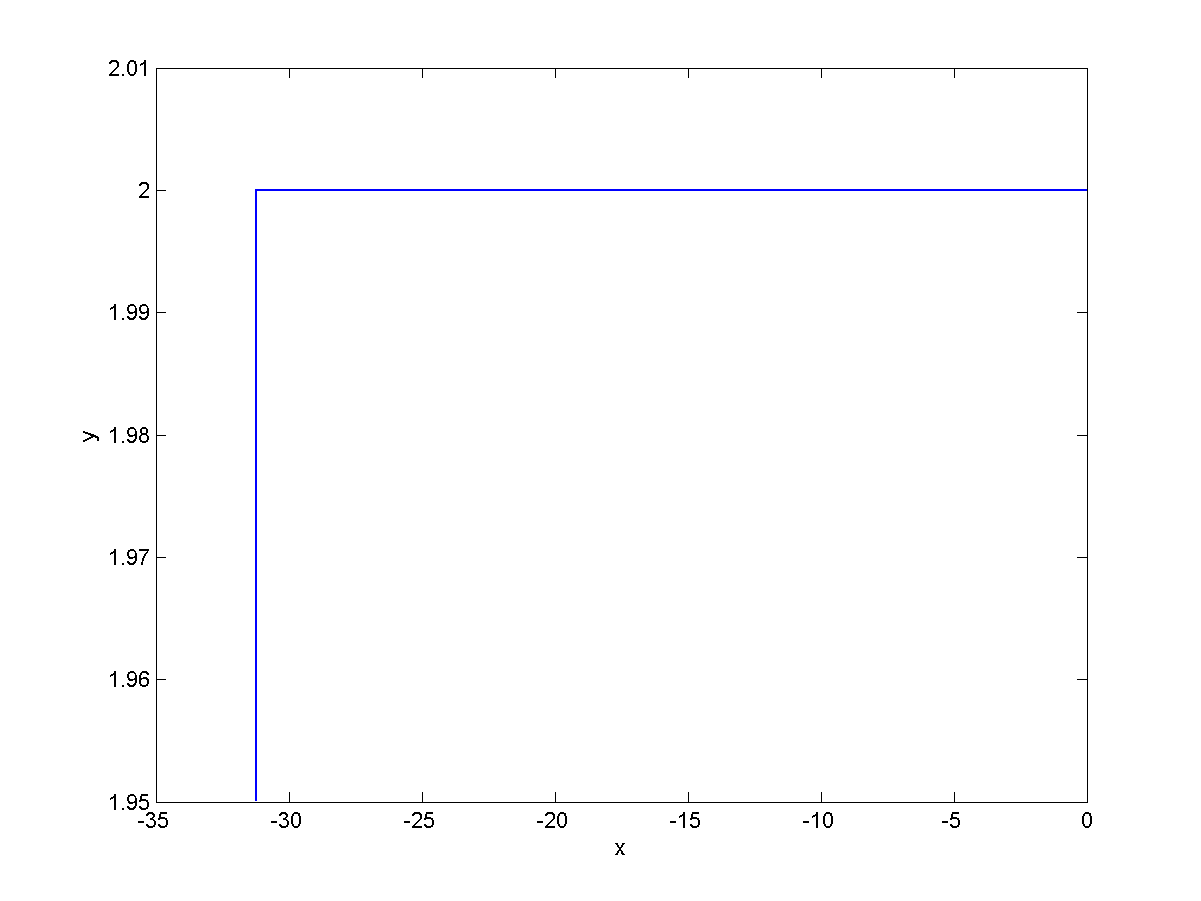
\includegraphics[width=\textwidth]{images/Q1_explicite_rate_p.png}
    \caption{$p$ pour explicite}
    \label{fig:q1_explicite_rate_p}
  \end{subfigure}
  ~
  \begin{subfigure}[b]{0.3\textwidth}
    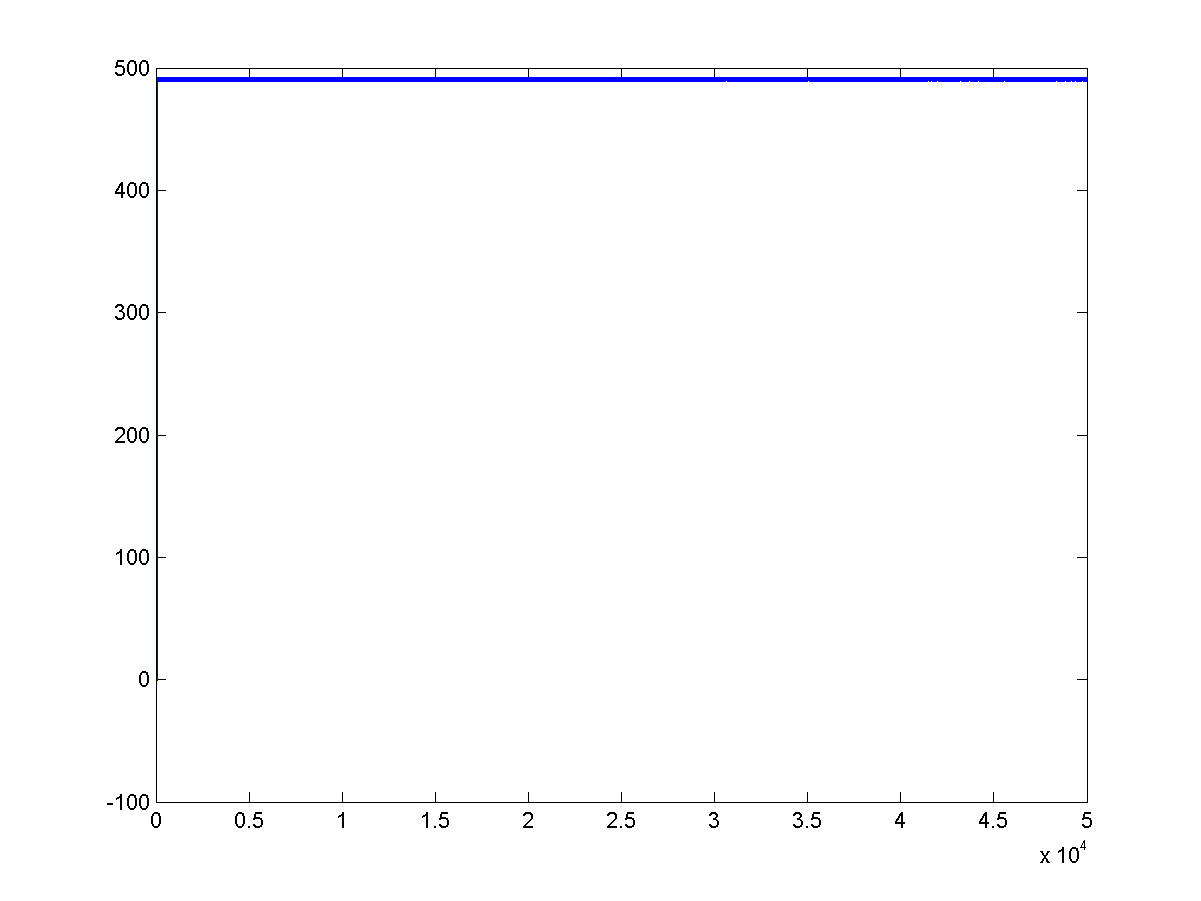
\includegraphics[width=\textwidth]{images/Q1_explicite_rate_H.png}
    \caption{$\Ha$ pour explicite}
    \label{fig:q1_explicite_rate_H}
  \end{subfigure}
\caption{Solutions de l'intégration numérique avec Euler explicite pour un pas $h=5$.}
\label{fig_rater}
\end{figure}

\subsubsection{Erreur}
L'erreur est par définition la différence entre la solution exacte et la solution obtenue par intégration numérique.
Comme nous ne disposons pas de la solution exacte, nous ne pouvons pas utiliser cette définition. Cependant, nous pouvons utiliser le graphe de $\Ha$.
En effet, nous savons que la solution exacte est telle que $\dot{\Ha} = 0$ ou autrement dit $\Ha$ ne varie pas avec le temps (d'une itération à l'autre).
Or sur la figure \ref{fig:q1_explicite_H}, on remarque que $\Ha$ augmente puis se stabilise une première fois à une certaine valeur (pour Euler explicite autour de $-0.495$ alors que la valeur initiale se situe à $-0.5$). Ensuite $\Ha$ ré-augmente encore et se re-stabilise encore à une valeur de $\Ha$ plus haute... on obtient une fonction $\Ha$ en escalier montant. Tandis qu'il diminue puis se stabilise une première fois autour d'une certaine valeur ($-0.505$) pour Euler implicite. Et on obtient une fonction en escalier descendant.
On peut interpréter cela de la manière suivante.
Le système d'équations différentielles \ref{equation_mvt} possède une infinité de solutions qui forment une famille de solutions.
Avec une condition initiale, on obtient alors une unique solution (si la condition de Lipschitz est satisfaite).
Lorsqu'on intègre numériquement ce système avec les méthodes d'Euler,
on commet forcément des erreurs qui, d'une itération à l'autre, peuvent
nous faire en quelques sorte passer d'une courbe de cette famille de solutions à une autre.
Ainsi sur la figure \ref{fig:q1_explicite_H} on passe d'une courbe de la famille de solution à une autre pour ensuite se stabiliser au alentour d'une solution (pour laquelle $\Ha=-0.505$) qui n'est pas la vraie solution,
mais qui en est à une distance constante. Ensuite, on fait un tour d'orbite et on rechange de courbe de solution (une qui a une énergie plus haute pour Euler explicite)... et on s'éloigne progressivement de la vraie solution (comme on s'en éloigne en augmentant d'énergie, les orbites sont de plus en plus de grande envergure). Si on met cela en lien avec la figure \ref{fig:q1_explicite_lambda} (partie réelle de $h\lambda$ en fonction du temps), on remarque que les endroits où on change d'orbite (où le $\Ha$ monte d'un étage) correspondent aux temps où les valeurs de $h \lambda $ sont grandes, c'est à dire les ``pics d'instabilités numériques''. \\
Pour Euler implicite (figure \ref{fig:q1_implicite_H}),
c'est la même chose, sauf qu'on stabilise autour d'une autre courbe de cette famille de solution (pour laquelle $\Ha = -0.495$), et à chaque tour d'orbite on rechange de courbe de solution pour aller vers une qui a une énergie $\Ha$ moindre (les orbites sont de plus en plus de petites envergures).\\
Pour le cas d'Euler symplectique, étant donné que le pas vaut $h=5 \cdot 10^{-2}$, les 100000 itérations nous emmènent plus loin dans le temps.
À chaque fois que l'on repasse près du point de départ,
on change de courbe dans la famille de solutions (on oscille donc autour de la vraie solution,
à une distance qui reste stable et relativement petite
\footnote{On observe que Euler symplectique commet une erreur sur le $\Ha$ qui est plus grande que celle commise par Euler implicite ou explicite sur une orbite (on oscille ici entre $-0.4$ et $-0.54$).
Cela est du au fait que la discrétisation temporelle est plus grossière.
D'ailleurs si on applique Euler symplectique avec $h=5.10^{-4}$, on obtient un $\Ha$ dont la valeur oscille entre $-0.495$ et $-0.505$, qui est l'erreur commise par Euler explicite/implicite sur la première revolution.}).\\
Dans le cas d'un pas de temps beaucoup trop grand comme dans la figure \ref{fig_rater},
on va aussi s'écarter de la vraie solution pour se stabiliser autour d'une courbe de la famille de solutions
(l'erreur reste alors constante, cf. figure \ref{fig_rater}), mais à une distance beaucoup plus grande de la vraie solution!



\subsubsection{Temps de calcul}
La méthode d'Euler explicite demande simplement d'évaluer les fonctions $f_1(p)$ et $f_2(q)$ à chaque itération.
Alors que la méthode d'Euler implicite exige à chaque itération,
de résoudre une équation non-linéaire.
%Le nombre d'itérations demandées à Newton-Raphson est illustré à la figure \ref{IterNR}.

%\begin{figure}
%\centering
%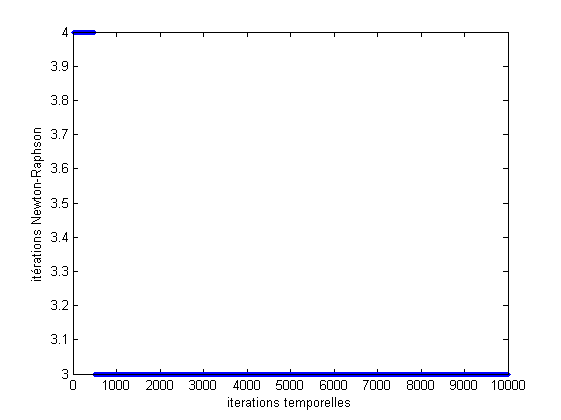
\includegraphics[width=7cm]{images/iterationNR.png}
%\caption{Nombre d'itérations nécessaire pour que Newton-Raphson converge.}
%\label{IterNR}
%\end{figure}

Les méthodes d'Euler symplectique ne demande pas plus de temps de calcul que celle d'Euler explicite. En effet, comme $f_1$ ne dépend que de $p$ et $f_2$ que de $q$, Euler symplectique consiste simplement à faire le calcul d'une des deux fonctions $p_{k+1}$ ou $q_{k+1}$ avec un Euler explicite, puis d'utiliser cette mise à jour d'une des deux fonctions pour calculer la deuxième. \\
Le temps de calcul pris par chaque méthode est indiqué dans la table \ref{table_time}.

\begin{table}[h]
\centering
\begin{tabular}{|c|cccc|}
\hline
 & Euler explicite & Euler implicite & Euler symplectique 1 & Euler symplectique 2 \\
\hline
Temps $[s]$ & 0.592897 & 254.122866 & 0.609895 &  0.605592\\
\hline
\end{tabular}
\caption{Temps de calcul pour les différentes méthodes avec 100 000 itérations temporelles.}
\label{table_time}
\end{table}

Comme prévu, les méthodes d'Euler explicite et symplectique demande un temps de calcul similaire. Celui d'Euler implicite est sensiblement plus élevé. Cela est du au fait que chaque itération temporelle demande trois itérations de Newton-Raphson dont chacune nécessite la résolution d'un système linéaire 4 sur 4.


\subsubsection{Conclusion} En théorie, le seul avantage de la méthode d'Euler implicite sur les autres est le fait qu'elle soit inconditionnellement stable. Cependant, on peut douter de l'intérêt d'utiliser une méthode inconditionnellement stable lorsqu'on résout une équation instable. D'ailleurs, si on applique Euler implicite avec un pas trop grand ($h=5.10^{-2}$, par exemple), on diverge tout autant qu'avec Euler explicite. \\
  Les méthodes symplectiques semblent être les plus avantageuses. En effet, bien qu'elles soient d'ordre 1 tout comme Euler implicite et explicite, elle donnent des résultats correctes pour un pas de temps $h=5.10^{-2}$, contrairement aux deux autres. Intuitivement, en comparant les figure \ref{fig:q1_explicite_H} et \ref{fig:q1_implicite_H}, on remarque que Euler implicite part dans un sens alors que l'explicite part dans l'autre. Comme la méthode symplectique fait une combinaison des deux, intuitivement, on peut supposer que les erreurs se corrigent en quelque sorte l'une l'autre.

  La méthode d'Euler symplectique est en fait souvent utilisée dans des problèmes comme celui-ci impliquant un hamiltonien. En effet elle évite ce qu'on appelle l'\textit{energy drift} qui est présent notamment dans le cas d'Euler explicite ou implicite, c'est à dire que l'énergie change de manière graduelle au cours du temps, comme cela apparait aux graphes \ref{fig:q1_explicite_H} et \ref{fig:q1_implicite_H}. Pour Euler symplectique, l'énergie va certes fluctuer mais restera comprise entre des bornes comme illustré aux graphes \ref{fig:q1_symplectique1_H} et \ref{fig:q1_symplectique2_H}.
